\section{Why do we embed networks?}
\label{sec:ch6:why}

Networks by themselves can have interesting properties, but a network is not how you traditionally organize data in computer science. In almost any ML algorithm - whether you're using a neural network or a decision tree, whether your goal is to classify observations or to predict values using regression - you'll see data organized into a matrix, where the rows represent observations and the columns represent features, or variables. In Section \ref{sec:ch1:whatis}, we called this data format \textit{tabular data}. 

Each row of this matrix is typically taken to be a unique ``piece'' of data, your observation. The columns typically are referred to as the ``features'', or are the elements of your data that you want to find relationships between. When this matrix has more than one feature, a typical way to conceptualize this example is that each row of the matrix is a $d$-dimensional vector (the dimensionality $d$ just means the number of features). These observations are often taken to be \textit{independent}, which informally means that the observations are not inter-related. 

By studying tabular data a little more in-depth, we can start to better understand a major challenge posed when learning from network data: underlying statistical dependencies.

\begin{floatingbox}[h]\caption{Lobster dataset}
To better understand the concepts of this section, we're going to go outside of network machine learning and try to understand a lobster dataset \cite{Sordalen2020Oct}. In this dataset, $n=2560$ lobsters were collected by a team of university investigators in Norway. For each lobster, the investigators measured the lobster's biological sex, the crusher claw width (CW), and the total length (TL) of the lobster, prior to release of the observed specimens (the features). Our question of interest is whether we can predict the crusher claw width using the lobster's biological sex and total length.
\end{floatingbox}

The key with this example is less the specific techniques that are applied, and more so the big picture of the implications of these problems on network data.

\subsection{Statistical dependence}

To visualize whether we might expect to find a relationship, we use a scatter plot, in Figure \ref{fig:ch5:lobster}. Each point represents the biological sex, CW, and TL of a single lobster. There is clearly a positive association, where longer lobsters tend to have larger crusher claws. Further, it would appear that male lobsters tend to have a much more dramatic increase in crusher claw width as total length increases. This data is encoded in a tabular format, where each row indicates the observation for a single lobster, and there are three columns (crusher claw width, total length, and biological sex). 

\begin{figure}[h]
    \centering
    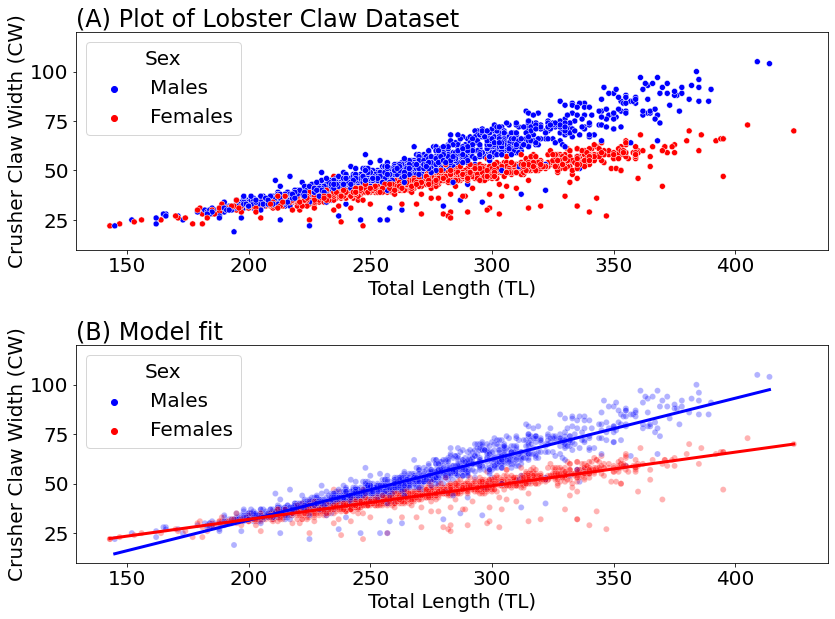
\includegraphics[width=0.7\linewidth]{representations/ch6/Images/lobster.png}
    \caption[Lobster example]{\textbf{(A)} a scatter plot of lobster total length against crusher claw width, separated by biological sex (shape). \textbf{(B)} a linear regression of the crusher claw width onto total length and biological sex, with an interaction term for biological sex and total length. Notice that the lines capture the dependence that we intuitively determined from \textbf{(A)}.}
    \label{fig:ch5:lobster}
\end{figure}


Conceptually, what this graph indicates is that there is likely a dependence in the dataset: crusher claw width appears to be related to both lobster total length (note that the larger lobsters tend to have greater claw widths) and biological sex (as males grow, their claw widths tend to increase faster than female claws).

If you remember back to traditional machine learning, it looks like you could fit a line between the total length and the crusher claw width for each lobster biological sex, and get a pretty good description of the relationship between the three features. Therefore, a first-pass strategy would be to use a linear regression. In this case, based purely on the information we have gathered from visualizing the data, an appropriate model would be a model which regresses the crusher claw width onto the lobster biological sex and total length (we think that biological sex and total length are informative about crusher claw width), and allow for the biological sex to modify the relationship between total length and crusher claw width (males have a steeper increase in crusher claw width with increasing size). 

You can see the results of this regression model that we have described in Figure \ref{fig:ch5:lobster}(B). It appears as though are relatively straightforward linear regression model does a fairly good job of capturing what we can intuitively derive from visualizing the data in Figure \ref{fig:ch5:lobster}(A). In this sense, we were able to explicitly describe a dependence that we expected, model it (using linear regression), and then capture it by fitting a regression model we believed to be appropriate.

As a caveat, it is almost never this easy to study a dependence, but it is often at least {possible} to do. The key that you should pick up on is that the traditional approach to dealing with dependencies when they arise in machine learning is to model them directly (like we did above) or indirectly (using latent models, an approach we did not describe here, but you can learn about in \cite{Hastie2009}). When we have underlying dependencies in the data and want to account for them, our approach is to explicitly describe or isolate the dependence whenever possible. Further, if we are uncertain about dependencies in the model, we can often do a pretty good job of inferring them.



\subsection{Why does this simple example indicate a problem with networks?}

This example, while trivial, gives us a good sense of some of the problems we're going to run into very quickly when we try to analyze network data. 

\subsubsection{Embedding is a tool to give you a tabular data structure}

All of the machine learning techniques and intuitions that you have probably built up through your education are most likely designed for tabular data formats. Networks are clearly not tabular at all; an observed network is a matrix and not a vector. It is unclear how exactly you can adapt your network to allow you to learn in the tabular setting you are more comfortable with. In this sense, an embedding is first and foremost a tool. Embedding is the ``bridge'' which provides functionality you need (namely, turning an adjacency matrix into a tabular format) so that you can churn them through the machine learning algorithms you are familiar with from elsewhere on your network data. You can embed your network, and doing nothing else, answer questions you might have about it. 

\subsubsection{Embedding provides an intuitive bridge when considered using statistical models}

All networks have the exact type of statistical dependence which arose in the lobster data, but on a much larger scale. When studying a dataset with $2$ features there is one possible dependence that can arise: the first feature can be related to the second feature. When studying a dataset with $3$ features like above, there are three possible dependencies that can arise: the first feature being related to the second, the second related to the third, and all three being inter-related. As you build up this logic, the number of possible dependencies with $d$ features winds up being $\frac{d!}{2}$, where $d!$ is the factorial operation $d\cdot (d - 1) \cdot (d - 2) \cdot ... \cdot 1$. When $d$ is small, this is extremely manageable with explicit modelling (like we did above for the lobsters). Even when $d$ is fairly large, it's typically the case that most of these dependencies are negligible.

Unfortunately for networks, this problem amplifies quickly. Remember that the adjacency matrix for a network is a collection of nodes and edges. Just thinking about this data structure inherently reveals a big problem to us: each edge depends on a pair of nodes, so our network has {at least} $\frac{n!}{2}$ dependencies we will need to at least consider when determining how to learn from the network. Stated another way, any pair of nodes could be correlated (because of the edges themselves), and further, nodes could be related to one another explicitly (by a specific grouping, such as a community assignment) or implicitly (by the nodes having similarities depending on different aspects of them that aren't immediately apparent at first glance). We will touch on both of these aspects a bit more in the next paragraph. To give you an indication of the scope of this problem, $\frac{n!}{2}$ is much bigger than $\binom n 2$, which we learned in Figure \ref{fig:ch4:nnets} is already an untenably large number even for modest choices of $n$. When $n$ is just $15$, this means there are about $10^{12}$ possible dependencies that may exist in the network.

\paragraph*{Explicitly delineating the dependence structure}

Sometimes, we can take the easy way out with network data, like we might do with tabular data: we can simply ignore a lot of the dependencies that might exist. If we think that there the nodes of our network are totally unrelated, we can learn from our network by using strategies appropriate for $ER_n(p)$ random networks. Remember that the $ER_n(p)$ random network made the assumption that all pairs of nodes had an equal connection probability (namely, $p$) which did not depend on any aspect of the individual nodes themselves. 

If we are given some sort of a grouping between the nodes, such as a community assignment vector, we can learn from the network using strategies appropriate for $SBM_n(\vec z, B)$ random networks. Remember than the $SBM_n(\vec z, B)$ random network model made the assumption that, once you know the community assignment of a pair of nodes node (given by $\vec z$), the edge probability was simply the appropriate entry of the block matrix. These approaches make excellent first-pass techniques for networks, and can be combined with other techniques we will see arise in the Part \ref{p:app} to learn lots of interesting facets of your dataset.

\paragraph*{If we can't explicitly delineate dependencies, what are we left with?}

The problem with networks that you might come across in your work is that they often won't fit into the scope of questions that you can ask with techniques that fall into this landscape where we can explicitly delineate out dependence structures immediately. 

You might have a network where you don't know a good grouping of the nodes ahead of time, or you might want to learn appropriate groupings of nodes directly from your data. You might think that there are dependencies that go beyond just a grouping of the nodes, or you might think that grouping your nodes together is inappropriate entirely. In this sense, there are a variety of ways in which prescriptive applications of SBMs with known community assignment vectors and ERs are not entirely appropriate.

 This massive problem of  where the opportunity and excitement of network machine learning comes into play. To overcome these problems, one of the primary tools that we will leverage is known as an embedding. An \textit{embedding} is a structure contained within another structure: in our case, we will attempt to find tabular structure that exists within our network and that we can analyze to describe our network.

\newpage